\subsubsection{Context and Context Conditions}
\label{context}

In this work we are interested in conditions related with the computing environment. These conditions are related with availability of computing resources, e.g. take a game that can be rendered using CPU or GPU, the availability of GPU is a contextual condition that restrict the achievement of goal render game using GPU strategy.
Adopting the context model proposed in \cite{ali_goal-based_2010} we will express such conditions as formulae in a set of facts. A given context satisfy a context condition if all related facts are monitored and the formulae associated are true.

The facts can be of an atomic proposition such as GPU, that is evaluated to true if an associated resource are known to be available, and it is evaluated to false otherwise.
The facts can be also logical conditions using logical operators ==, !=, <, <=, >, >=.


\subsubsection{Goals, Components and Artifacts}
\label{sec:rules}

We enhance enhance component description with context condition. We extend Yu et al.\cite{yu_goals_2008} patterns for the Goals-Component view with contextual conditions.

\begin{table}[]
\centering
\caption{Contextual Goal Model to components; (1) context condition, (2) And-decomposition, (3)OR-decomposition}
\label{table_related_works}
\begin{tabular}{|l|l|}
\hline
 %\textbf{ A } & \textbf{ B} & \textbf{C} \\ \hline
 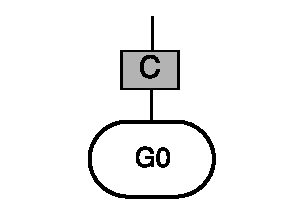
\includegraphics[scale=0.5]{patterns_condition} &
 \begin{lstlisting}
 Component G0 {
   provides IG0;
   condition C;
 }
 \end{lstlisting} \\ \hline
 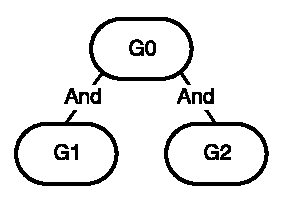
\includegraphics[scale=0.5]{patterns_and_decomposition} &
 \begin{lstlisting}
 Component G0 {
   provides IG0;
   requires IG1, IG2;
 }
 \end{lstlisting} \\ \hline
 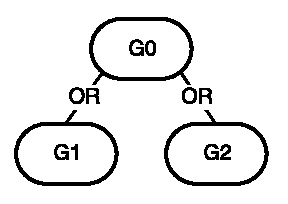
\includegraphics[scale=0.5]{patterns_or_decomposition} &
 \begin{lstlisting}
 Component G1 {
   provides IG0;
 }
 Component G2 {
   provides IG0;
 }
 \end{lstlisting} \\ \hline
\end{tabular}
\end{table}

Software component should be packaged in a standard packaging schema.
The package should, also, have meta-data describing goals it provides, context conditions, and dependencies.

Artifact is a tupla (component, metadata) and metadata is a tupla (context conditions, dependencies, provided goals) context, goals and dependencies.

\begin{itemize}
  \item Context conditions can be evaluated against the context. If the conditions are not satisfied the machine should not deploy the component.
  \item Dependencies are required services that should be provided by other components. Before deploy the component the machine should verify if it can satisfy the dependencies of the component.
  \item Provided goals are services that the component provide to the user or to other components.
\end{itemize}

The artifact dependency: all that its components depend
The artifact provide:  all that its components provide
The artifact conditions:  all that its components conditions

If both context conditions and dependencies are satisfied, the artifact is capable of allow the goal achievement.

\subsubsection{Online Goals}

In traditional goal modeling the agent have a root goal that are refined in subgoals.  Or-refinements allow for variability points in the goal model, but that refinement are static, at least for a given version of the goal model.
We argue that in a dynamic and open environment that vision is not sufficient. We propose a different vision for the autonomous deployment. An agent should have a set of goals that it should pursue. That set can be updated by and user or the agent itself when following a self-assembly approach~\cite{sykes_flashmob:_2011}. We call \emph{active goal} a goal that the agent must pursue.
In a dynamic environment, the agent can at a given moment have or not the resources to achieve a goal. \emph{Achievable Goal} is a goal that the agent pursue and is capable of achieve.

In our deployment view of the goals, we will consider a goal achievable if we can deploy at least one artifact that provide that goals.

\subsubsection{Evolution}

evolve without great effort.

We argue that a goal model can be seen as a protocol definition. When we create OR-Refinements we are giving alternatives of execution, creating variability points.

By creating interfaces in variability points
Open deployment platform.

  and we create opportunity for thirty-parties provide new alternativies

having different context condition will allow the goal to be achievable in a broader range of contexts: for example, in screen controls will allow the game to be playable at touch screen devices.

In tradition deployment schema, a complete new version of the software should be released.

\begin{figure}[!htb]
  \centering
  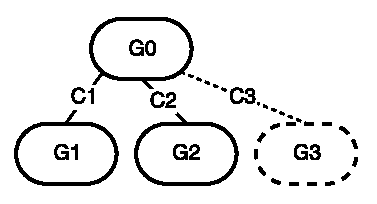
\includegraphics[width=\linewidth]{evolution_or}
  \caption{Evolution OR}
\label{fig:evolution_or}
\end{figure}

Component development and release
